\documentclass{beamer}
\usepackage{amsmath}   % For mathematical symbols
\usepackage{amssymb}   % For additional symbols
\usepackage{graphicx}  % For including images

% Simple theme and colors
\usetheme{Madrid}
\setbeamercolor{title}{fg=black}
\setbeamercolor{author}{fg=black}
\setbeamercolor{date}{fg=black}
\setbeamercolor{frametitle}{fg=white, bg=black}
\setbeamercolor{background canvas}{bg=white}
\setbeamertemplate{footline}[frame number] % Only show frame numbers

% Title page details
\title{\textbf{Two-Stage Object Detection}}
\author{\textbf{ANAND M K}}
\date{}

\begin{document}

% Title page slide
\begin{frame}
    \titlepage
\end{frame}

% Slide 2: Introduction to Object Detection
\begin{frame}{\textbf{Introduction to Object Detection}}
   \begin{itemize}
    \item \textbf{Image Classification:} 
      Takes an image and predicts the object in the image.
    \item \textbf{Object Localization:} 
      Locates the presence of an object in the image and represents it with a bounding box.
    \item \textbf{Object Detection:} 
      Combines image classification and object localization. It takes an image as input and produces one or more bounding boxes with the class label attached to each bounding box.
  \end{itemize}
  \vfill
  % Add the image here
  \begin{center}
      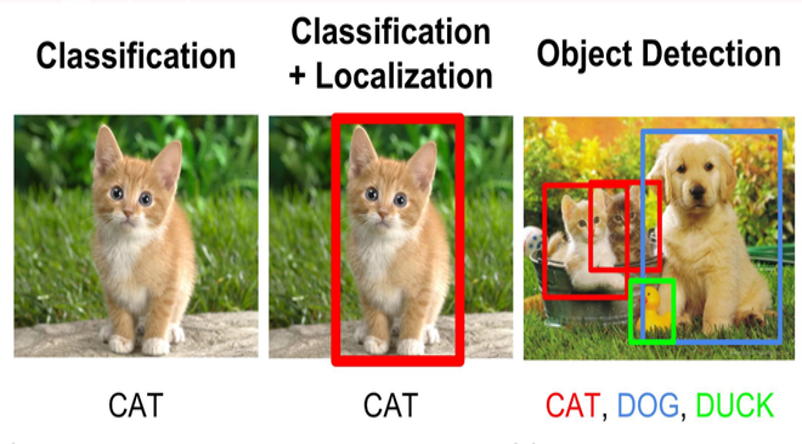
\includegraphics[width=0.6\textwidth]{Picture1.png}
  \end{center}
\end{frame}

% Slide: Single-Stage vs. Two-Stage Object Detectors (Image)
\begin{frame}{\textbf{Single-Stage vs. Two-Stage Object Detectors}}
  \begin{center}
      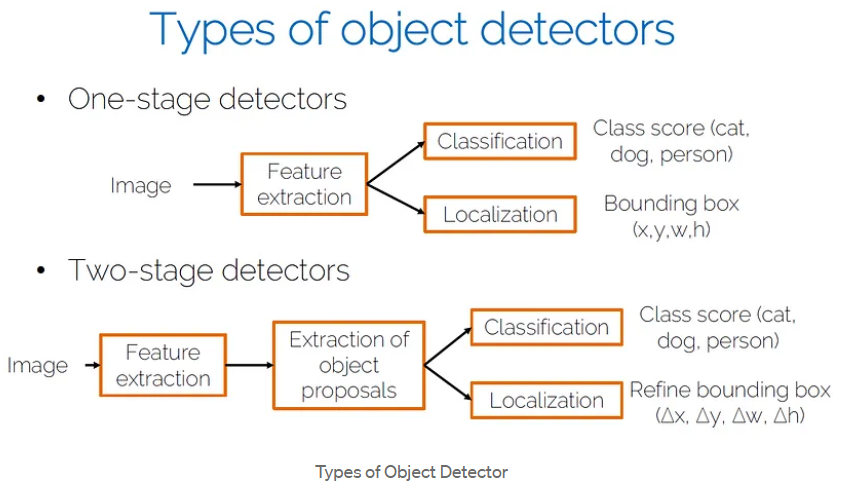
\includegraphics[width=0.8\textwidth]{slide2.png} % Use the image file name here
  \end{center}
\end{frame}
% Slide: Single-Stage vs. Two-Stage Object Detectors (Text)
\begin{frame}{\textbf{Single-Stage vs. Two-Stage Object Detectors}}
  \begin{itemize}
    \item \textbf{Single-Stage Object Detector:}
    \begin{itemize}
      \item Directly goes from the image to classification and bounding box coordinates.
      \item Features are extracted using a CNN, which are then used for classification and regression.
      \item \textbf{Advantages:}
      \begin{itemize}
        \item Very fast, suitable for real-time object detection.
      \end{itemize}
      \item \textbf{Disadvantages:}
      \begin{itemize}
        \item Performance can be poorer than two-stage detectors.
      \end{itemize}
      \item \textbf{Examples:} YOLO family, SSD, RetinaNet.
    \end{itemize}
    
    \item \textbf{Two-Stage Object Detector:}
    \begin{itemize}
      \item Divides the process into two steps:
      \begin{enumerate}
        \item Extracts features using a CNN.
        \item Extracts regions of interest (object proposals) for classification and localization.
      \end{enumerate}
      \item \textbf{Advantages:}
      \begin{itemize}
        \item Extremely accurate with high mean Average Precision (mAP).
        \item More suitable for applications where accuracy is prioritized over speed (e.g., medical imaging).
      \end{itemize}
      \item \textbf{Examples:} R-CNN family.
    \end{itemize}
  \end{itemize}
\end{frame}

% Slide: Two-Stage Object Detection
\begin{frame}{\textbf{Steps of Two-Stage Object Detection}}
  \begin{itemize}
    \item \textbf{Step 1: Region Proposal}
    \begin{itemize}
      \item The model uses a Region Proposal Network (RPN) to generate candidate regions, known as region proposals.
      \item These regions are likely to contain objects.
    \end{itemize}
    
    \item \textbf{Step 2: Classification and Bounding Box Refinement}
    \begin{itemize}
      \item Each proposed region is classified to determine the object category.
      \item The bounding box is adjusted to accurately surround the detected object.
    \end{itemize}
  \end{itemize}
  
  \vfill
  % Add the image of the flowchart here
  \begin{center}
    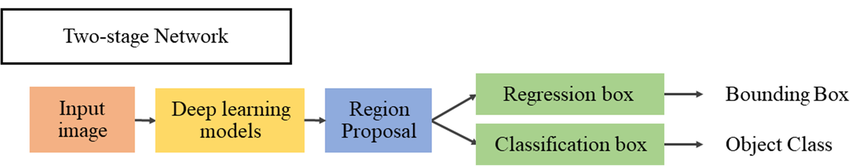
\includegraphics[width=0.9\textwidth]{slide3.png}
  \end{center}
\end{frame}



% Slide: Bounding Box Regression and Localization
\begin{frame}{\textbf{Localization: Bounding Box Regression}}
    \begin{itemize}
        \item Bounding Box Regression is the process of refining the predicted object location by learning four key coordinates: 
        \begin{itemize}
            \item \(x, y\) (center of the box)
            \item \(w, h\) (width and height of the box)
        \end{itemize}
        \item A CNN extracts features from the image and predicts the coordinates of the object.
        \item The goal is to minimize the difference between the predicted box and the ground truth box using a loss function, typically L2 loss.
    \end{itemize}
    
    \vfill
    % Add the image for visual representation
    \begin{center}
        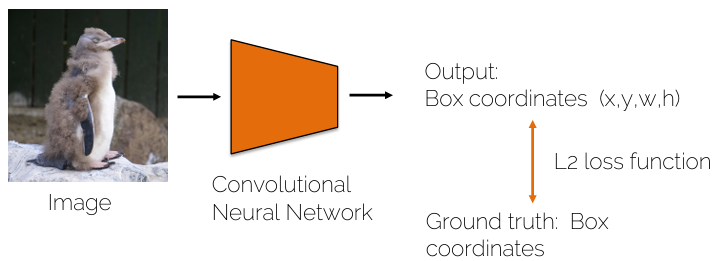
\includegraphics[width=0.9\textwidth]{slide4.png}
    \end{center}
   
\end{frame}

% Slide: Localization and Classification in Object Detection
\begin{frame}{\textbf{Localization and Classification}}
  \begin{itemize}

    \item \textbf{Classification:}
    \begin{itemize}
      \item The task is to classify the object in the bounding box.
      \item The CNN extracts features and uses fully connected layers to predict class scores.
      \item The loss function used for class score prediction is \textbf{Softmax loss}.
    \end{itemize}
  \end{itemize}

  % Add the image here
  \begin{center}
      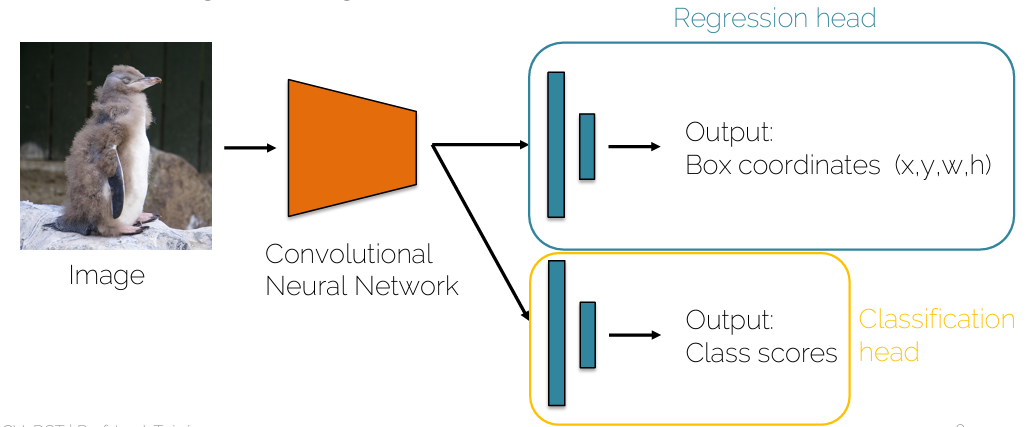
\includegraphics[width=0.8\textwidth]{slide5.png}
  \end{center}
\end{frame}

\begin{frame}{\textbf{R-CNN (Regions with Convolutional Neural Networks}}
    \begin{center}
        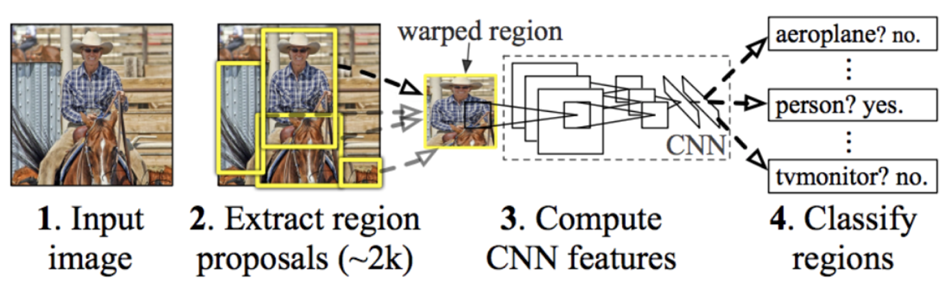
\includegraphics[width=1\textwidth]{slide6.png} % Region proposal and feature extraction image
    \end{center}
    \begin{itemize}
        \item \textbf{Step 1: Region Proposal Generation}
        \begin{itemize}
            \item Use selective search to generate around 2000 candidate regions.
        \end{itemize}
    \end{itemize}

\end{frame}

\begin{frame}{\textbf{R-CNN: Steps 2 and 3 (Feature Extraction and Classification)}}
    \begin{itemize}
        \item \textbf{Step 2: Feature Extraction}
        \begin{itemize}
            \item Resize each region to a fixed size and extract features using a CNN.
        \end{itemize}
        
        \item \textbf{Step 3: Classification and Bounding Box Regression}
        \begin{itemize}
            \item Classify each region proposal using an SVM (Support Vector Machine).
            \item Refine bounding box coordinates using linear regression.
        \end{itemize}
    \end{itemize}
    \begin{center}
        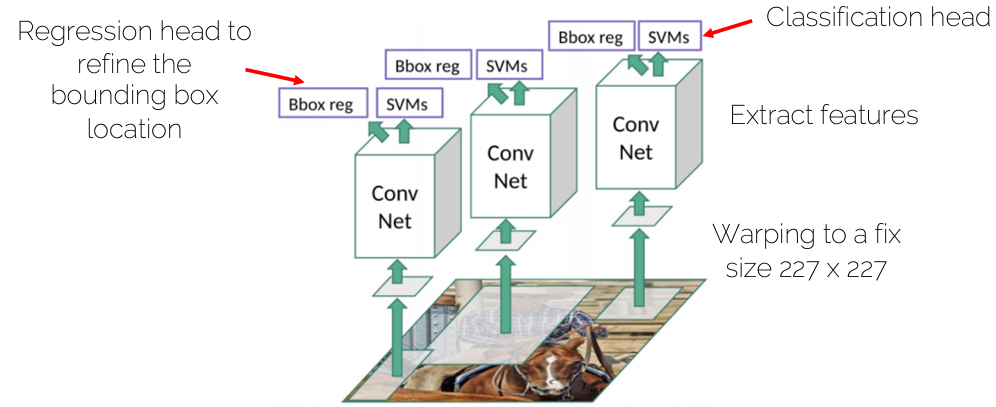
\includegraphics[width=0.9\textwidth]{slide7.png} % Classification, bounding box regression, and NMS image
    \end{center}
\end{frame}


\begin{frame}{\textbf{Selective Search for Region Proposals}}
    \begin{itemize}
        \item Selective Search is a region proposal algorithm used in object detection.
        \item It generates candidate object locations by grouping similar regions in an image.
    \end{itemize}
    \begin{center}
        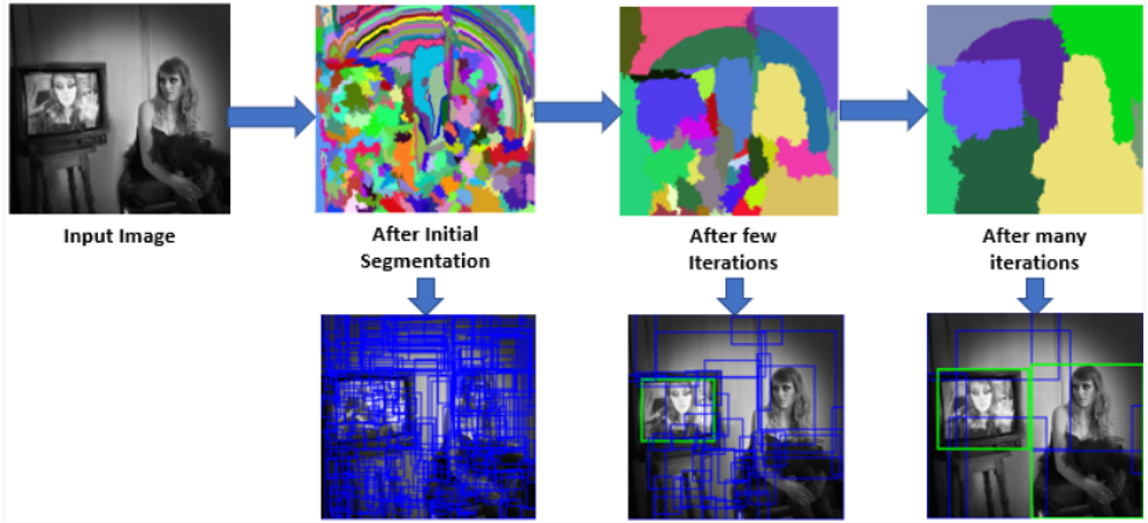
\includegraphics[width=1\textwidth]{slide8.png} % Replace with appropriate image file
    \end{center}
\end{frame}

\begin{frame}{\textbf{Selective Search for Region Proposals}}
    \begin{itemize}
        \item \textbf{Step 1: Over-Segmentation}
        \begin{itemize}
            \item Break the image into many small regions based on pixel color and intensity.
        \end{itemize}
        
        \item \textbf{Step 2: Initial Region Proposal}
        \begin{itemize}
            \item Treat each small region as a starting point for object candidates.
        \end{itemize}
        
        \item \textbf{Step 3: Merge Similar Regions}
        \begin{itemize}
            \item Combine neighboring regions that are similar in color, texture, size, and shape.
        \end{itemize}

        \item \textbf{Step 4: Generate Region Proposals}
        \begin{itemize}
            \item As regions merge, create larger candidate regions for potential objects.
        \end{itemize}
        
        \item \textbf{Step 5: Repeat Merging}
        \begin{itemize}
            \item Continue merging until the entire image is covered by larger regions, generating multiple proposals at different scales.
        \end{itemize}
    \end{itemize}
\end{frame}


\begin{frame}{\textbf{Limitations of R-CNN}}
    \begin{itemize}
        \item \textbf{Slow Processing Speed:}
        \begin{itemize}
            \item Each region proposal requires a separate forward pass through the object detector, making it resource-intensive and slow.
        \end{itemize}

        \item \textbf{Fixed Object Proposal Algorithm:}
        \begin{itemize}
            \item The use of a fixed selective search algorithm does not allow for improvement through training.
        \end{itemize}
        
        \item \textbf{Separate Training:}
        \begin{itemize}
            \item Feature extraction and SVM classifier are trained separately, limiting the model's ability to exploit learning potential.
        \end{itemize}
    \end{itemize}
\end{frame}


\begin{frame}{\textbf{Introduction to Fast R-CNN}}
    \begin{itemize}
        \item Fast R-CNN is an advanced object detection framework that enhances the original R-CNN approach.
        \item By employing a single forward pass through a convolutional neural network (CNN), it efficiently extracts features from the entire image, minimizing computational overhead.
    \end{itemize}
    \vfill
    % Add the image of Fast R-CNN here
    \begin{center}
        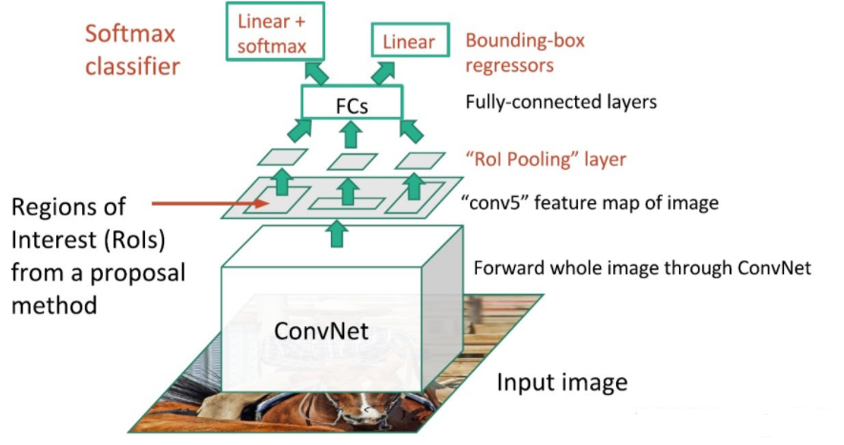
\includegraphics[width=0.8\textwidth]{slide9.png} % Replace with your image filename
    \end{center}
\end{frame}



\begin{frame}{\textbf{Overview of Fast R-CNN Working}}
    \begin{itemize}
        \item \textbf{Single Forward Pass:}
        \begin{itemize}
            \item Fast R-CNN processes the entire image through a convolutional neural network (CNN) in a single forward pass, generating a feature map.
        \end{itemize}

        \item \textbf{Region Proposal Generation:}
        \begin{itemize}
            \item An external algorithm (e.g., Selective Search) generates a set of candidate region proposals from the image.
        \end{itemize}

        \item \textbf{Region of Interest (RoI) Pooling:}
        \begin{itemize}
            \item The feature map is used to extract features for each region proposal.
            \item RoI pooling converts these features into a fixed size to enable processing by fully connected layers.
        \end{itemize}

        \item \textbf{Fully Connected Layers:}
        \begin{itemize}
            \item The pooled features are fed into fully connected layers for classification and bounding box regression.
        \end{itemize}

        \item \textbf{Output:}
        \begin{itemize}
            \item The softmax layer predicts class probabilities for each region.
            \item The bounding box regression layer refines the bounding box coordinates for more accurate localization.
        \end{itemize}
    \end{itemize}
    \vfill
\end{frame}

\begin{frame}{ROI Pooling: Key Concepts}

    \textbf{Feature Map:} 
    Dimensions \( L \times K \times C \), where \( L \times K \) is the spatial size and \( C \) is the number of channels.

    \textbf{Object Proposals:} 
    Define regions (green box) of interest in the feature map, which vary in size.
    
    \textbf{Problem:} 
    FC layers need fixed-size input \( H \times W \times C \).

    \vspace{0.4cm}
    \centering
    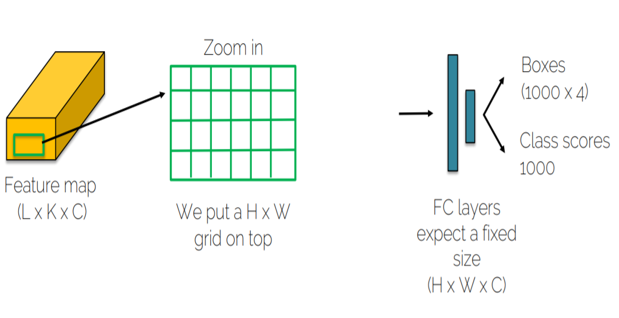
\includegraphics[width=0.8\linewidth]{slide10.png}

\end{frame}

\begin{frame}{ROI Pooling}

    \textbf{Pooling:} 
    A grid \( H \times W \) is placed over the region, and max-pooling is applied in each cell to produce a fixed-size \( H \times W \times C \) feature map.

    \textbf{FC Layer Input:} 
    The output is resized to fit the FC layers.
    
    \vspace{0.4cm}
    \centering
    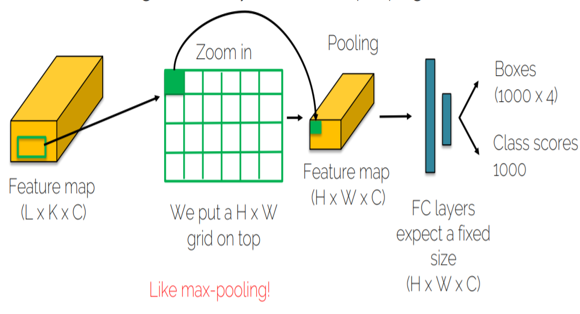
\includegraphics[width=0.8\linewidth]{slide11.png}

\end{frame}
\begin{frame}{\textbf{Challenges of Fast R-CNN}}
    \begin{itemize}
        \item \textbf{Selective Search Dependency:}
        \begin{itemize}
            \item Fast R-CNN uses Selective Search as a method for generating Regions of Interest (RoIs).
            \item This approach is inherently slow and time-consuming.
        \end{itemize}
        
        \item \textbf{Performance Issues:}
        \begin{itemize}
            \item Detection time is approximately 2 seconds per image, an improvement over R-CNN.
            \item However, in large real-life datasets, this speed may not be sufficient, making Fast R-CNN less effective.
        \end{itemize}
    \end{itemize}
\end{frame}

% Slide 1: Overview of Faster R-CNN with RPN
\begin{frame}
    \frametitle{Faster R-CNN}

    \begin{columns}
        % Left column for text
        \begin{column}{0.5\textwidth}
            \begin{itemize}
                \item Faster R-CNN is an extension of Fast R-CNN with a Region Proposal Network (RPN) that enhances speed and efficiency.
                \item RPN replaces traditional region proposal methods (Selective Search) with a fully convolutional network.
                \item RPN improves object detection by proposing regions (bounding boxes) directly from feature maps.
            \end{itemize}
        \end{column}

        % Right column for image
        \begin{column}{0.5\textwidth}
            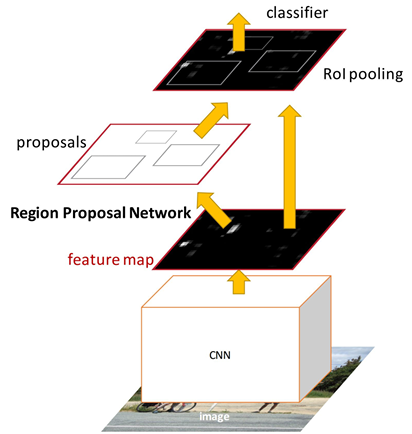
\includegraphics[width=\linewidth]{slide12.png} 
        \end{column}
    \end{columns}
\end{frame}


% Slide 1: Introduction to RPN
\begin{frame}
    \frametitle{Region Proposal Network (RPN) Overview}

    \begin{itemize}
        \item RPN generates region proposals (bounding boxes) directly from feature maps.
        \item RPN is fully convolutional and slides over feature maps to generate proposals for objects in the image.
    \end{itemize}
   
    \centering
    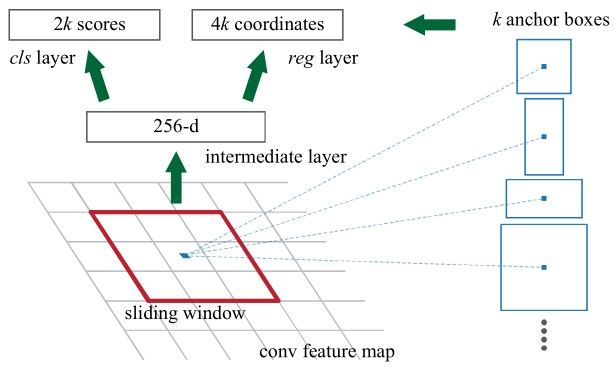
\includegraphics[width=0.8\linewidth]{slide14.jpg}

\end{frame}


% Slide 2: Detailed Working of RPN
\begin{frame}
    \frametitle{RPN - Working Mechanism}

    \begin{itemize}
        \item \textbf{Sliding Window:}
        \begin{itemize}
            \item RPN uses a sliding window that moves across the convolutional feature map to detect potential objects.
        \end{itemize}

        \item \textbf{256-d Intermediate Layer:}
        \begin{itemize}
            \item At each sliding window position, a 256-dimensional feature vector is extracted to capture visual information.
        \end{itemize}

        \item \textbf{k Anchor Boxes:}
        \begin{itemize}
            \item For each sliding window, \(k\) anchor boxes (default: 9) are generated with various scales and aspect ratios.
        \end{itemize}

        \item \textbf{2k Scores (cls layer):}
        \begin{itemize}
            \item The classification layer predicts whether each of the \(k\) anchor boxes contains an object (positive) or not (negative).
            \item The result is \(2k\) scores—two for each anchor box: one score for object presence and one for absence.
        \end{itemize}

        \item \textbf{4k Coordinates (reg layer):}
        \begin{itemize}
            \item The regression layer refines the bounding box coordinates for each anchor by predicting 4 values: (x, y, width, height).
            \item The result is \(4k\) coordinates for anchor box refinement.
        \end{itemize}
    \end{itemize}
\end{frame}

% Slide: Advantages of Faster R-CNN
\begin{frame}
    \frametitle{Advantages of Faster R-CNN}
    
    \begin{itemize}
        \item \textbf{Speed:} 
        \begin{itemize}
            \item Replaces traditional region proposal methods with a Region Proposal Network (RPN), significantly improving detection speed.
        \end{itemize}
        
        \item \textbf{Unified Framework:} 
        \begin{itemize}
            \item Integrates region proposal and object detection into a single network, streamlining the process and reducing computational overhead.
        \end{itemize}
        
        \item \textbf{Scalability:} 
        \begin{itemize}
            \item Capable of handling a large number of object categories without separate steps for region proposal and detection.
        \end{itemize}
        
        \item \textbf{Improved Accuracy:} 
        \begin{itemize}
            \item Jointly trained RPN and Fast R-CNN network improve localization and classification accuracy.
        \end{itemize}
    \end{itemize}
    
\end{frame}


% Slide: Conclusion
\begin{frame}
    \frametitle{Conclusion}

    \begin{itemize}
        \item Two-stage object detection algorithms like Faster R-CNN separate the process into region proposal and object classification, offering higher accuracy by refining object localization.
        \item The introduction of Region Proposal Network (RPN) significantly improved both speed and accuracy in the two-stage detection pipeline.
        \item While two-stage methods are generally more accurate, one-stage detectors (like YOLO, SSD) offer faster inference by directly predicting bounding boxes and class scores in a single step.
        \item Each approach has its own trade-offs between speed and accuracy, with Faster R-CNN excelling in applications requiring precise detection.
    \end{itemize}
    
\end{frame}




\end{document}
